\documentclass[letterpaper, 12pt]{article}
\usepackage[top=2cm,bottom=1cm,left=0.75in,right=0.75in,headheight=17pt, % as per the warning by fancyhdr
includehead,includefoot,
heightrounded, % to avoid spurious underfull messages
]{geometry}
\addtolength{\topmargin}{-.25in}
\usepackage{fancyhdr}
\pagestyle{fancy}
\usepackage{graphicx}
\usepackage{lastpage}
\usepackage{pgfplots}
\pgfplotsset{width=10cm,compat=1.9}

\begin{document}
\fancyhead[l]{	\includegraphics[height=1cm]{"../../Templates/Year C/club".png} Name:}
\fancyhead[r]{Due Date \hspace{ 1in}}
\cfoot{\thepage\ of \pageref{LastPage}}
	

	
\begin{center}Assignment 1.01: Density
\end{center}

\begin{enumerate}




	\item You are thinking about buying a water bed to use in your second-floor bedroom.  The dimensions of the water bed are 1.83 m x 2.13 m x 0.229 m.  The floor can tolerate a weight of no more than 6660 N. Find the weight of the water in the bed, and determine if you should purchase this bed.
	\vspace{1in}
		
	\item The United States Nickle has remained largely unchanged from 1938 to the present (with the exception of the 2004 and 2005 commemorative nickles), whereas pennies have been made from bronze, brass, aluminum, steel and copper-plated zinc.  Explain why some someone would want to use a nickle to test if a scale is accurate and not a penny.  
	\vspace{1in}
	
	\item The Georgia state capital is covered in gold leaf (gold that has been pounded into a thin sheet), with a thickness of 3 x 10\textsuperscript{-7} m.  The dome is a half-sphere with a diameter of 22.86 meters.  Find the mass of the gold that covers the dome.  The density of gold is 19320 kg/m\textsuperscript{3}.  
	\vspace{1in}
		
	\item The sun has a radius of 6.96 x 10\textsuperscript{8} m, and a mass of 1.998 x 10\textsuperscript{30} kg.  Saturn has a radius of 6 x 10\textsuperscript{7} m, and a mass of 5.7 x 10\textsuperscript{26} kg.  Imaging that there were an enormous ocean, capable of holding the Sun and Saturn at the same time.  
	\begin{enumerate} 
		\item Would the sun float or sink?  Justify your answer.
		\vspace{0.5in}
		\item Would Saturn float or sink?  Justify your answer.
	\end{enumerate}
	\vspace{1in}
	
	\item You are given a sample of and unknown fluid and are asked to determine the fluid the sample is made of.  You are given the following information:
		\begin{center}
			\begin{tabular}{ | c | c | }
				\hline
				Substance & Density ($kg / m^3$) \\ \hline
				Gasoline & 711 \\ \hline
				Extra Virgin Olive Oil & 785.1 \\ \hline
				Water & 1000 \\ \hline
				Whole Milk & 1020 \\ \hline
				Ethelyne Glycol & 1120 \\ \hline
				Sodium Hydroxide  & 1250 \\ \hline
			
		
				\end{tabular}
		\end{center}
		
		You collect the information in the table below:
		\vspace{.1in}
		

		\begin{tabular}{ | c | c | }
			\hline
			Volume (mL) & Mass (g) \\ \hline
			20 & 50.702 \\ \hline
			40 & 66.404 \\ \hline
			60 & 82.106 \\ \hline
			80 & 97.808 \\ \hline
			100 & 113.51 \\ \hline
			120  & 129.212 \\ \hline
			140  & 144.914 \\ \hline
			160  & 160.616 \\ \hline			
			180  & 176.318 \\ \hline			
			200  & 192.02 \\ \hline			
			
		\end{tabular}
		
		\vspace{-2.5in} 
		\hspace{2.5in}
		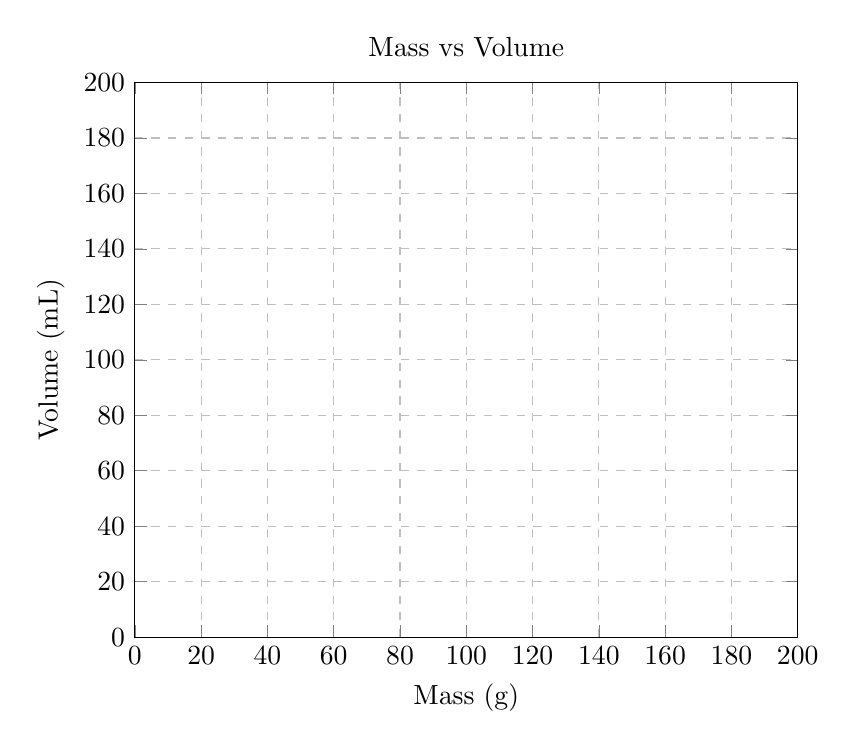
\begin{tikzpicture}
		\begin{axis}[
		title={Mass vs Volume},
		xlabel={Mass (g)},
		ylabel={Volume (mL)},
		xmin=0, xmax=200,
		ymin=0, ymax=200,
		xtick={0,20,40,60,80,100,120,140,160,180,200},
		ytick={0,20,40,60,80,100,120,140,160,180,200},
		legend pos=north west,
		ymajorgrids=true,
		xmajorgrids=true,
		grid style=dashed,
		]
	
		
		
		\end{axis}
		\end{tikzpicture}
		
		\begin{enumerate}
			\item On the graph to the right, plot the data you have collected.  Draw a best fit line and determine the slope of the line. 
			\vspace{0.4in}
			
			\item Use the slope of the line to determine the density of the fluid, and determine which fluid is most likely present in the sample. 
			\vspace{0.4in}
			
			\item Briefly explain what physical quantity the y-intercept of the graph represents.
		
		\end{enumerate}

	
	
	
\end{enumerate}
 



\end{document}
